% Section 3.3 insertion; the existing introduction is retained.
Using the mixture model in Equation~\ref{eq:mixpdf1}, we compare predicted
completeness and contamination with direct counts from the cleaned HST sample
for $24\leq r<24.5$ and $24.5\leq r<25$
(Figure~\ref{fig:singleband-prediction-comparison}). At $p_S>0.2$, V10 predicts
contamination of 11.1\% and 47.6\% in the two intervals, whereas HST measures
48.1\% and 77.8\%, respectively.

To investigate this discrepancy, we also test a core-plus-tail model for the
unresolved component.
\begin{equation}
 U_{\rm cpt}(\Delta m_r\mid m)=A\left[(1-\epsilon)G(\Delta m_r\mid m)
                 +\epsilon\,(G*E_\tau)(\Delta m_r\mid m)\right].
 \label{eq:singleband-core-tail}
\end{equation}
Here $G$ is a Gaussian with center and magnitude-dependent width fixed by an
earlier $r$-only calibration; $E_\tau$ is an exponential distribution of
nonnegative offsets with mean $\tau$; and $*$ denotes convolution. The total
unresolved fraction is $A$, of which $\epsilon$ belongs to the tail. We also
refit the resolved density, which integrates to $1-A$ and can be nonzero near
$\Delta m_r=0$ (Figure~\ref{fig:singleband-component-comparison}). In each interval,
we minimize the mean negative log-likelihood of the $r$ photometry plus
$0.001\,A\epsilon$.

\begin{samepage}
In both target intervals, the core-plus-tail model gives closer
contamination predictions at $p_S>0.2$: it predicts 49.4\% and 64.8\%, and
HST measures 53.9\% and 76.4\% for its selections. The absolute prediction
differences fall from 37.0 to 4.5 percentage points in the brighter interval
and from 30.2 to 11.6 percentage points in the fainter interval. Its predicted
completeness is also closer to HST at this threshold.

\end{samepage}

XXXXXX:Could ZI add more work on 3.3?


Closer prediction does not establish better stellar selection at all
completeness levels. When the same model family is fitted separately at fainter magnitudes, the population ratio departs from the COSMOS2020 reference. For
$25.5\leq r<26$, the fitted resolved-to-unresolved ratio is approximately
2.4, compared with 33 from V10 and 49 in the COSMOS2020 reference.

The core-plus-tail model is used here as an $r$-band comparison. For the
subsequent multiband $D$ analysis, particularly $griz$, we retain the V10
stellar width $\sigma_U(m)$. Further investigation of the population
decomposition using independent information, for example from Gaia and Roman,
is left to future work.

XXXXXX:ZI can add more details about the future plan.

XXXXXX: Could ZI check all the plots captions in the paper? I think some captions are too long...

\begin{figure*}[!htbp]
\centering
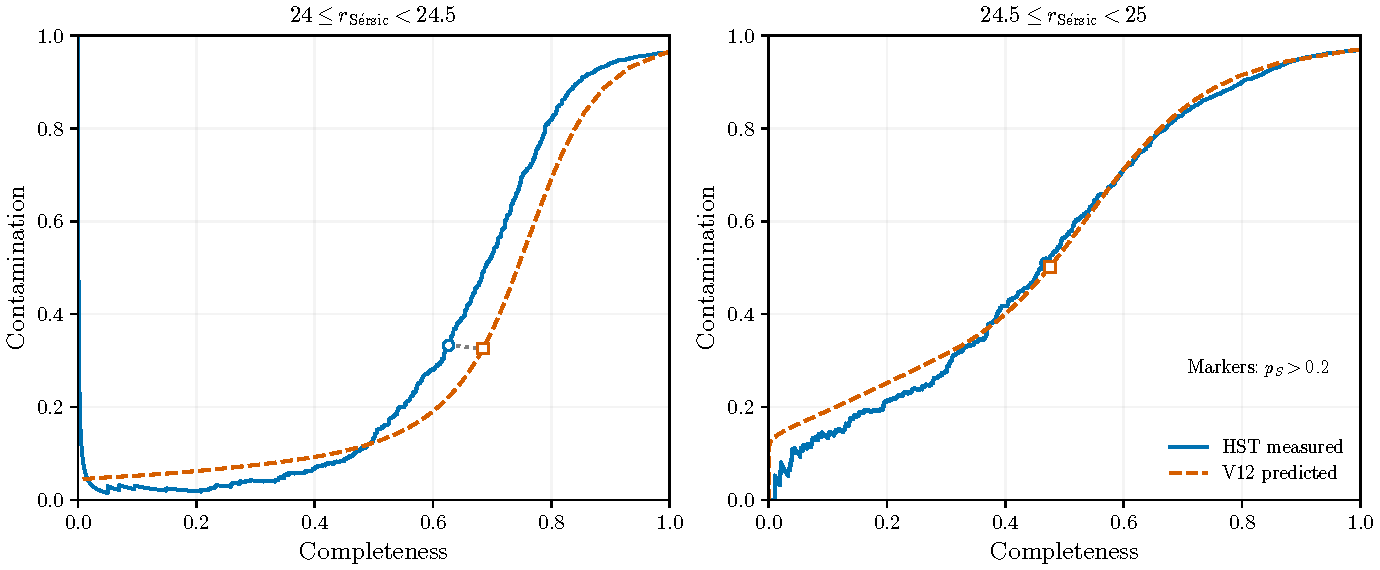
\includegraphics[width=\textwidth]{posterior_prediction.pdf}
\caption{Model-predicted and HST-measured completeness--contamination relations for the V12 $r$-band probability. Columns show $24\leq r<24.5$ and $24.5\leq r<25$. Blue curves use HST counts; orange dashed curves integrate the weighted V12 components over the full $p_S$ selection at each magnitude. Circles and squares mark $p_S>0.2$ in the HST and model results. The samples contain 1,319 stars and 36,129 galaxies, and 1,636 stars and 50,780 galaxies, respectively; both use $-0.5<\Delta m_r<1.5$.}
\label{fig:singleband-prediction-comparison}
\end{figure*}

\begin{figure*}[!htbp]
\centering
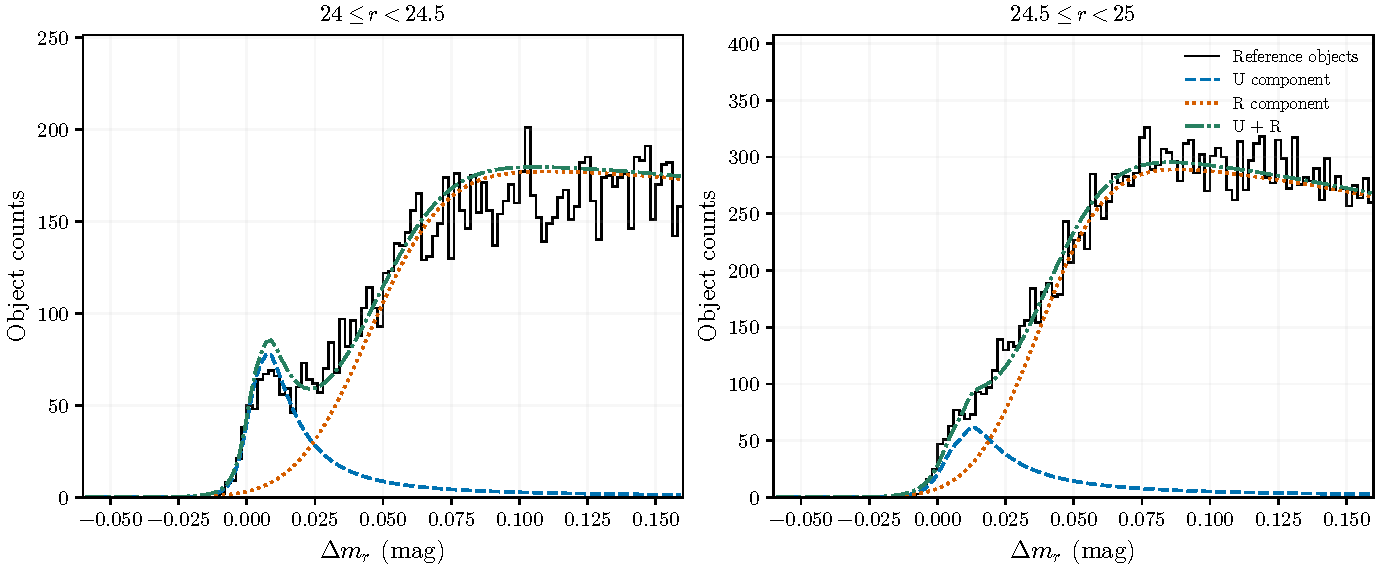
\includegraphics[width=\textwidth]{posterior_components.pdf}
\caption{Observed $r$-band $\Delta m$ counts of the accepted reference cohort (black) and the V12 U, R, and total expected counts (blue dashed, orange dotted, and green dash-dotted). Columns show $24\leq r<24.5$ and $24.5\leq r<25$. Expectations integrate the densities within each histogram bin and average over the measured magnitudes; their full normalization uses $-0.5<\Delta m_r<1.5$. The positive U wing is distinct from the narrow core used to define $D$.}
\label{fig:singleband-component-comparison}
\end{figure*}

\begin{figure*}
\centering
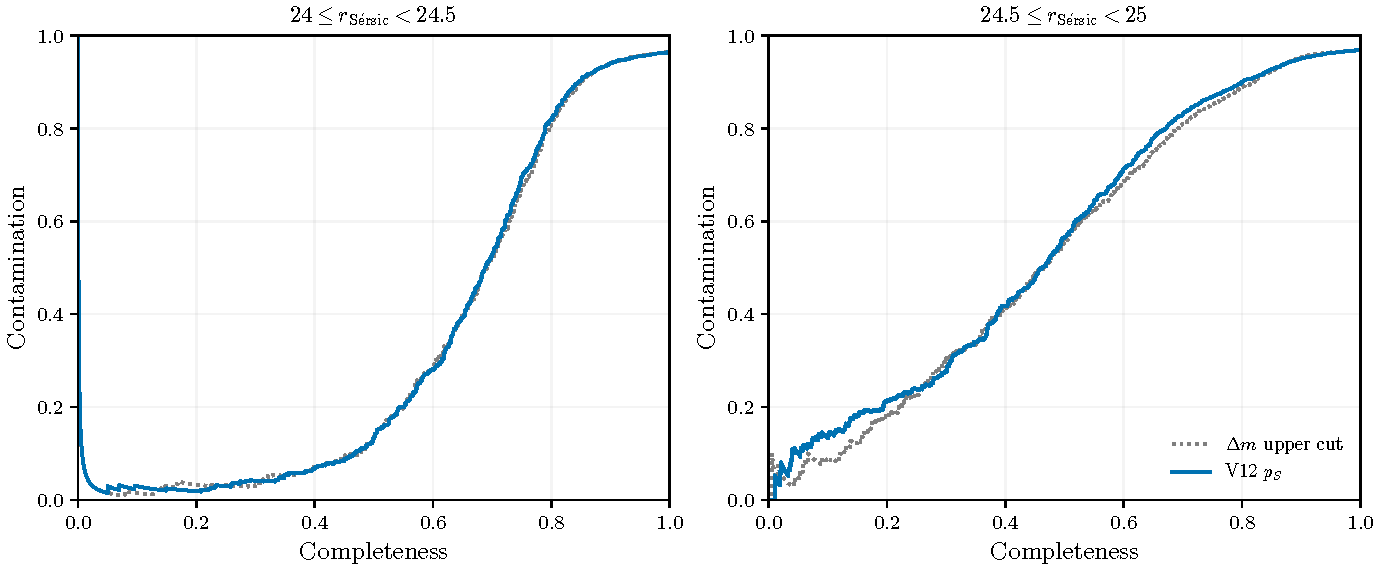
\includegraphics[width=\textwidth]{posterior_selection.pdf}
\caption{HST-measured selection performance for a signed $\Delta m_r$ upper cut (gray dotted) and V12 $p_S$ (blue solid), on the same finite-support reference objects as Figure~\ref{fig:singleband-prediction-comparison}. Every attainable score threshold is retained in the calculation. The two rankings use different information: $p_S$ includes both fitted densities and their magnitude-dependent fractions.}
\label{fig:singleband-selection-comparison}
\end{figure*}



% Keep the comparison figures before the next subsection in this preview.
\clearpage
